\section{Instalación de Oracle Server} 
\vspace{\baselineskip}
Luego de ingresar con el usuario “oracle”, abrimos el archivo “oracle s Home” del escritorio, de donde borramos la carpeta “database”. 
\begin{center}
	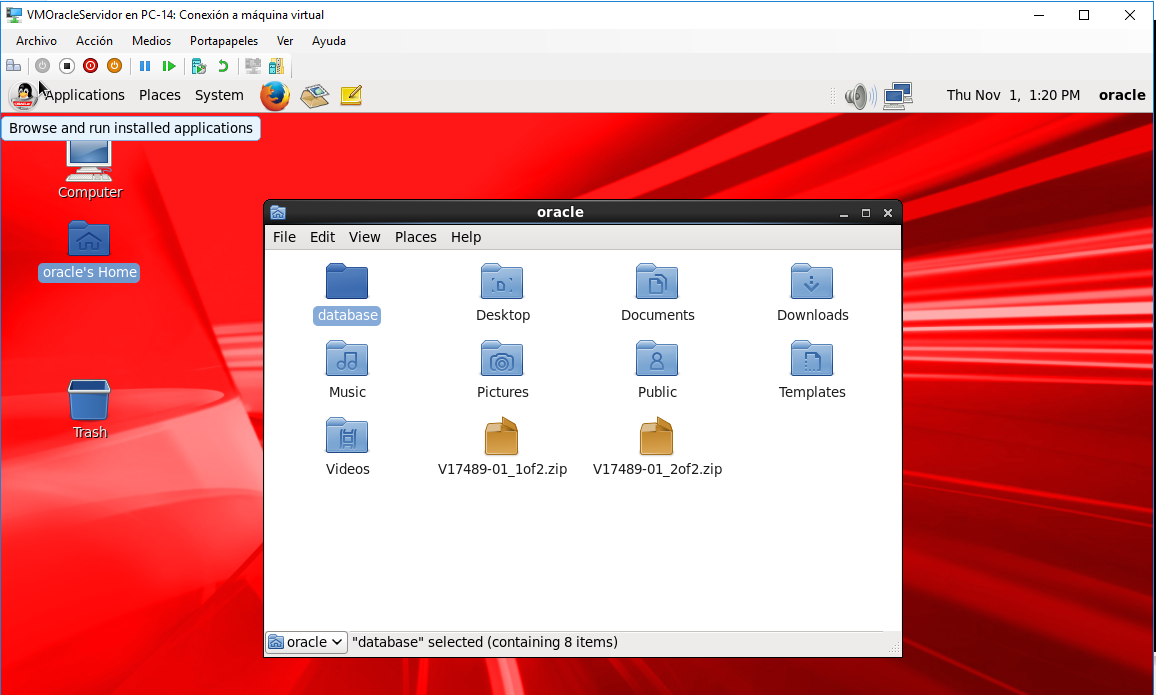
\includegraphics[width=16cm]{./Imagenes/57} 
\end{center} 

\vspace{\baselineskip}

Luego abrimos el archivo llamado “V17489-01 lof.zip”
\begin{center}
	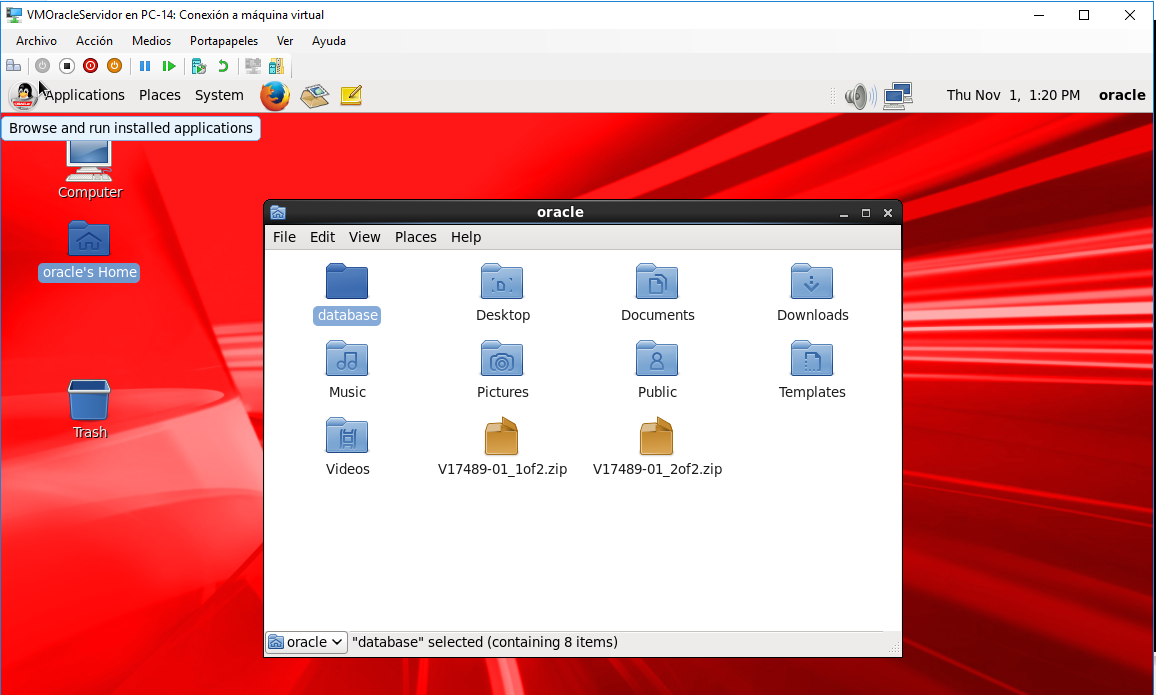
\includegraphics[width=16cm]{./Imagenes/58} 
\end{center} 

\vspace{\baselineskip}

Dentro del archivo, presionamos el botón “Extract”.
\begin{center}
	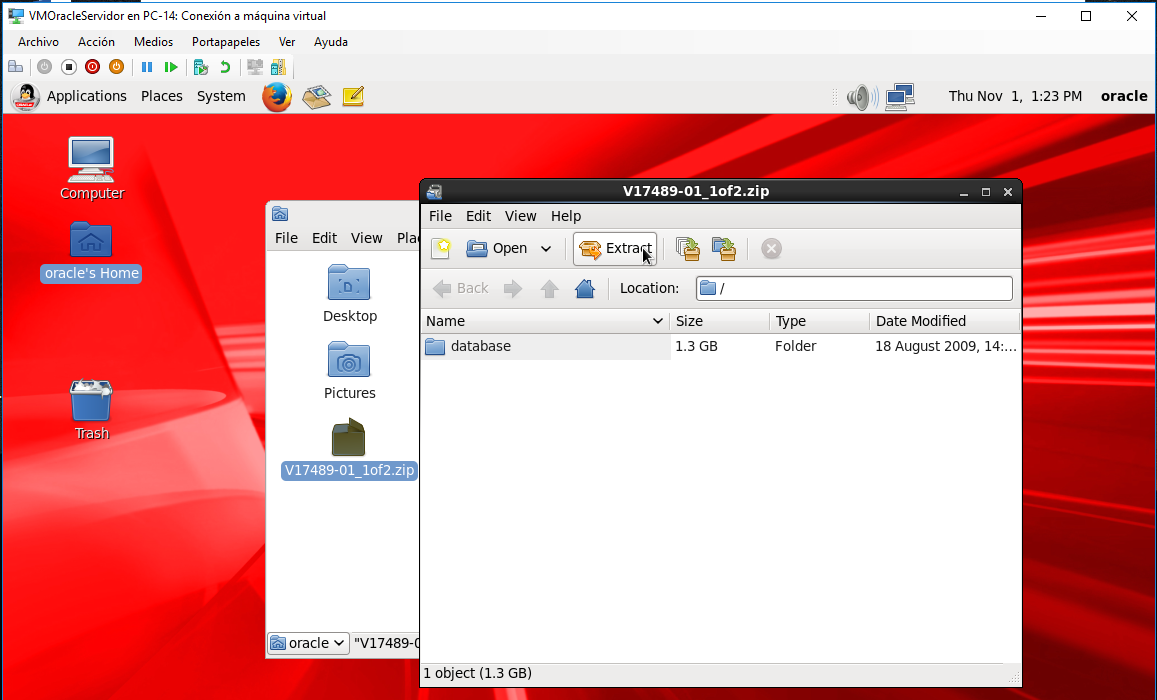
\includegraphics[width=16cm]{./Imagenes/59} 
\end{center} 

\vspace{\baselineskip}

Se nos aparecerá la siguiente ventana, en donde presionamos el botón “Extract”.
\begin{center}
	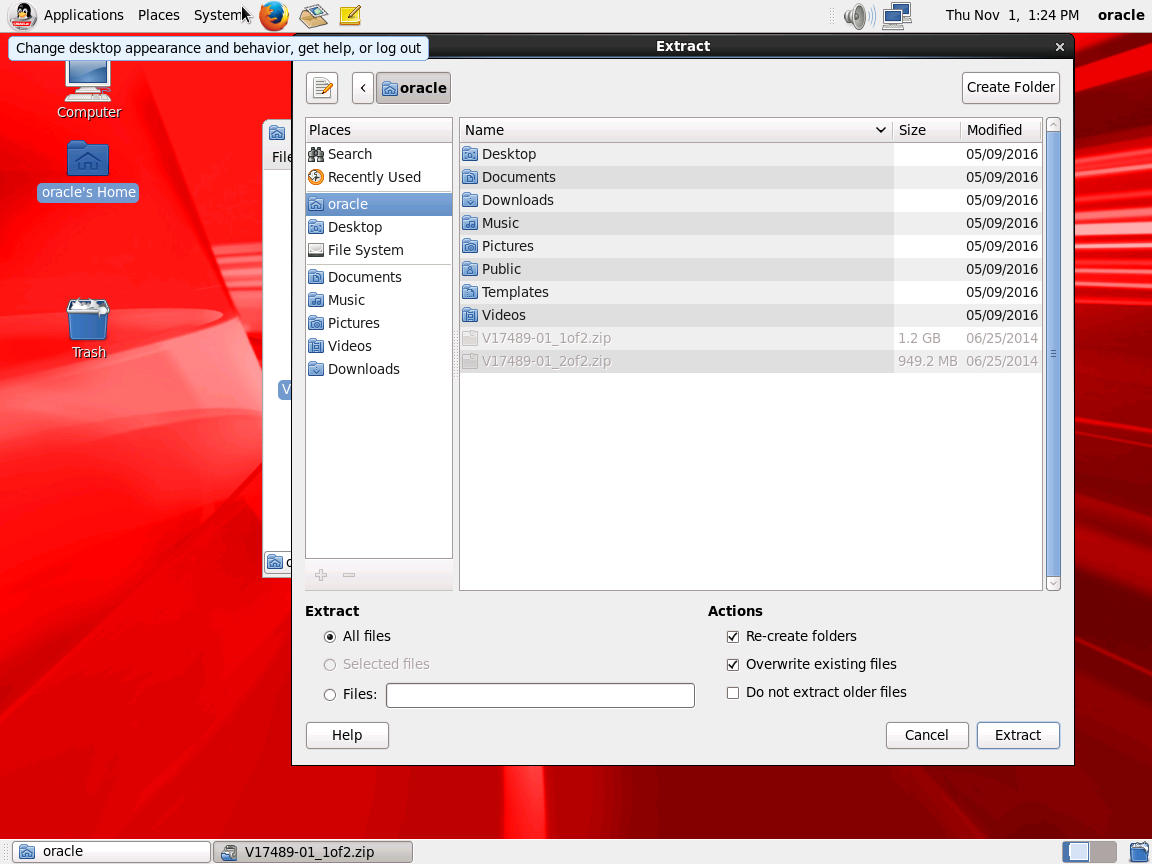
\includegraphics[width=16cm]{./Imagenes/60} 
\end{center} 

\vspace{\baselineskip}

Seguidamente comenzara a extraer todos los ficheros del archivo seleccionado, esperamos a que termine el proceso.
\begin{center}
	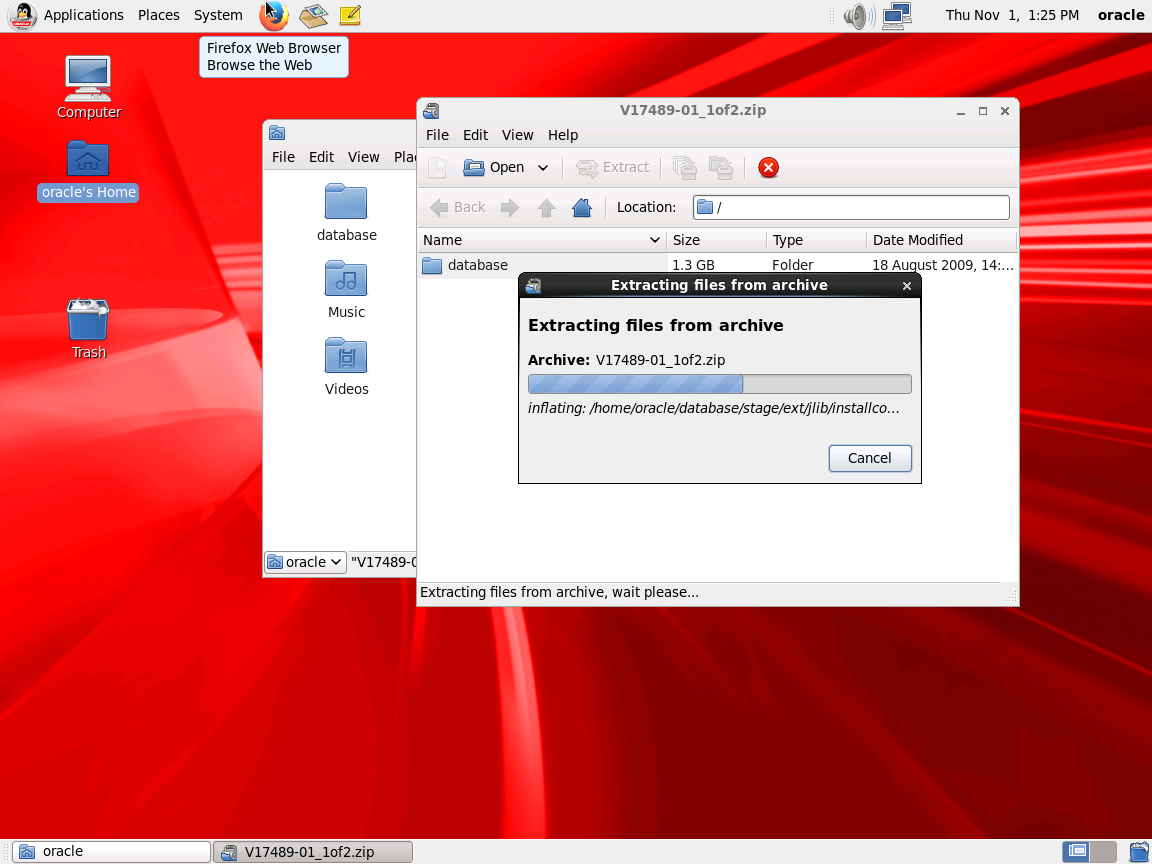
\includegraphics[width=15cm]{./Imagenes/61} 
\end{center} 

\vspace{\baselineskip}

Realizamos los mismo para el siguiente archivo llamado “V17489-01 2lof.zip”
\begin{center}
	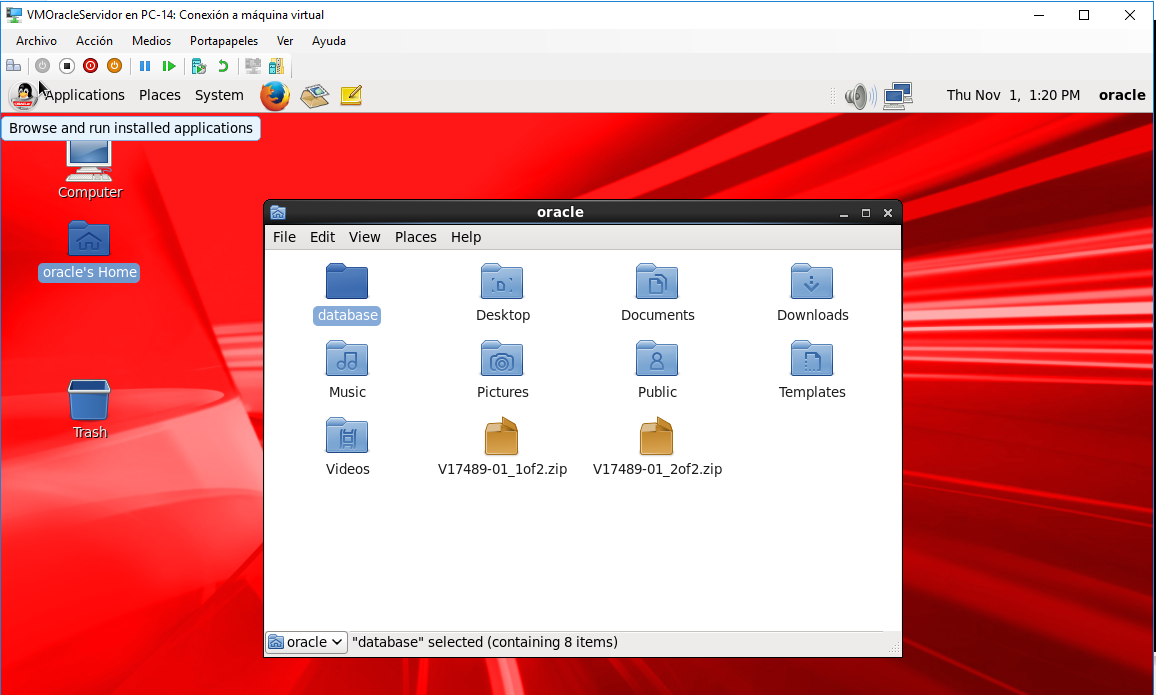
\includegraphics[width=15cm]{./Imagenes/62} 
\end{center} 

\vspace{\baselineskip}

Dentro del archivo, presionamos el botón “Extract”.
\begin{center}
	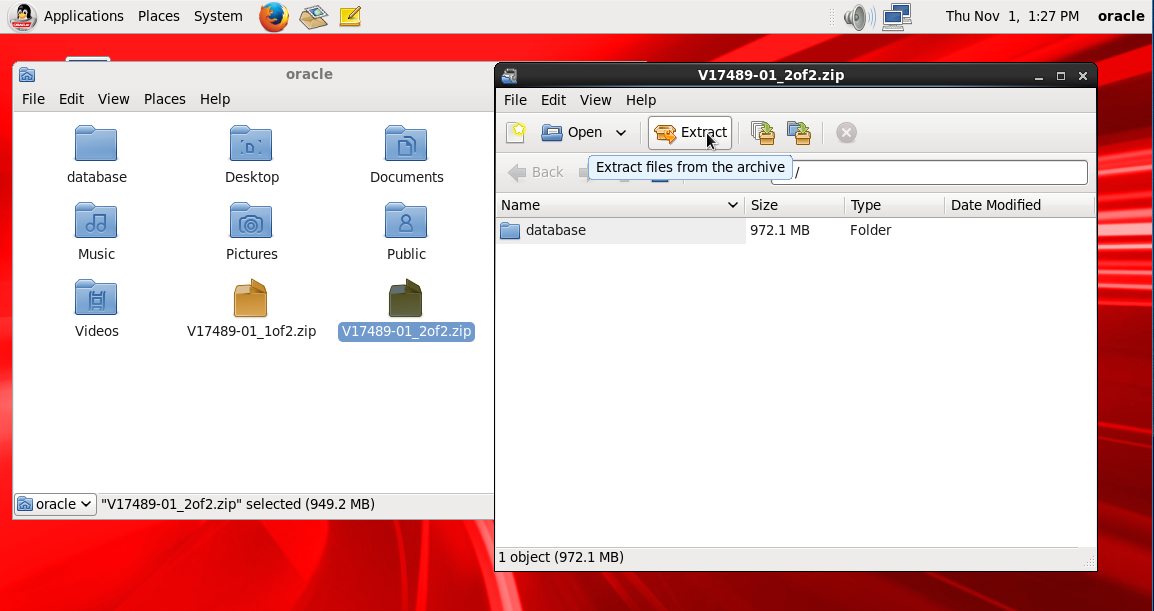
\includegraphics[width=16.5cm]{./Imagenes/63} 
\end{center} 

\vspace{\baselineskip}

Se nos aparecerá la siguiente ventana, en donde presionamos el botón “Extract”.
\begin{center}
	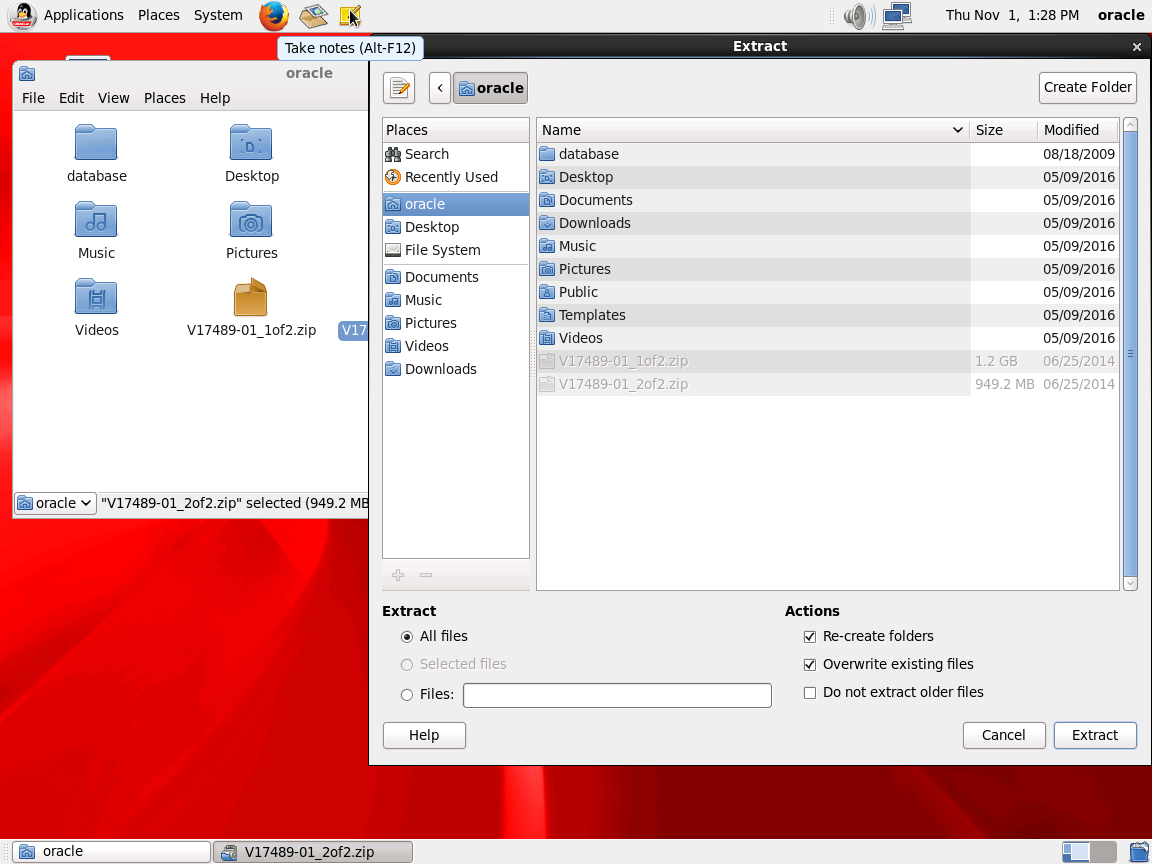
\includegraphics[width=16.5cm]{./Imagenes/64} 
\end{center} 

\vspace{\baselineskip}

Seguidamente comenzara a extraer todos los ficheros del archivo seleccionado, esperamos a que termine el proceso.
\begin{center}
	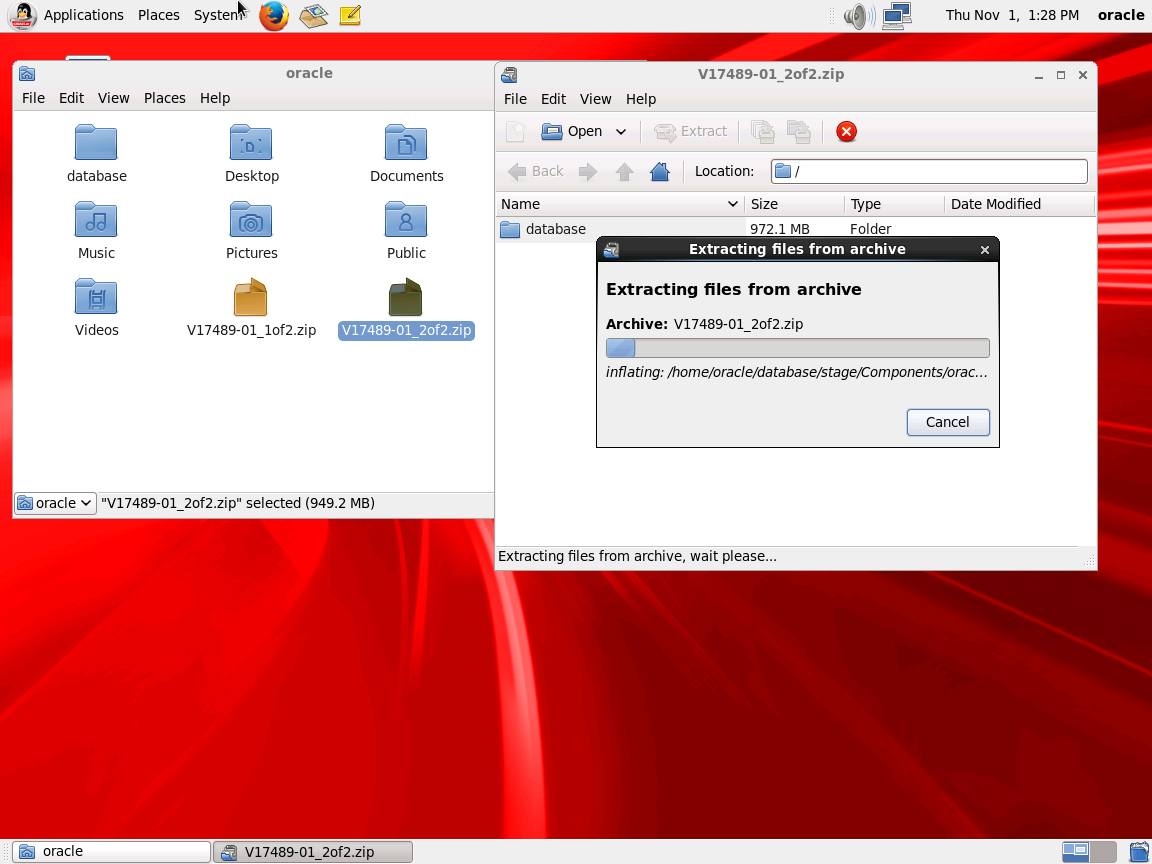
\includegraphics[width=15cm]{./Imagenes/65} 
\end{center} 

\vspace{\baselineskip}

Seguidamente observamos que se nos ha creado una carpeta denominada “database”, en la cual ingresamos.
\begin{center}
	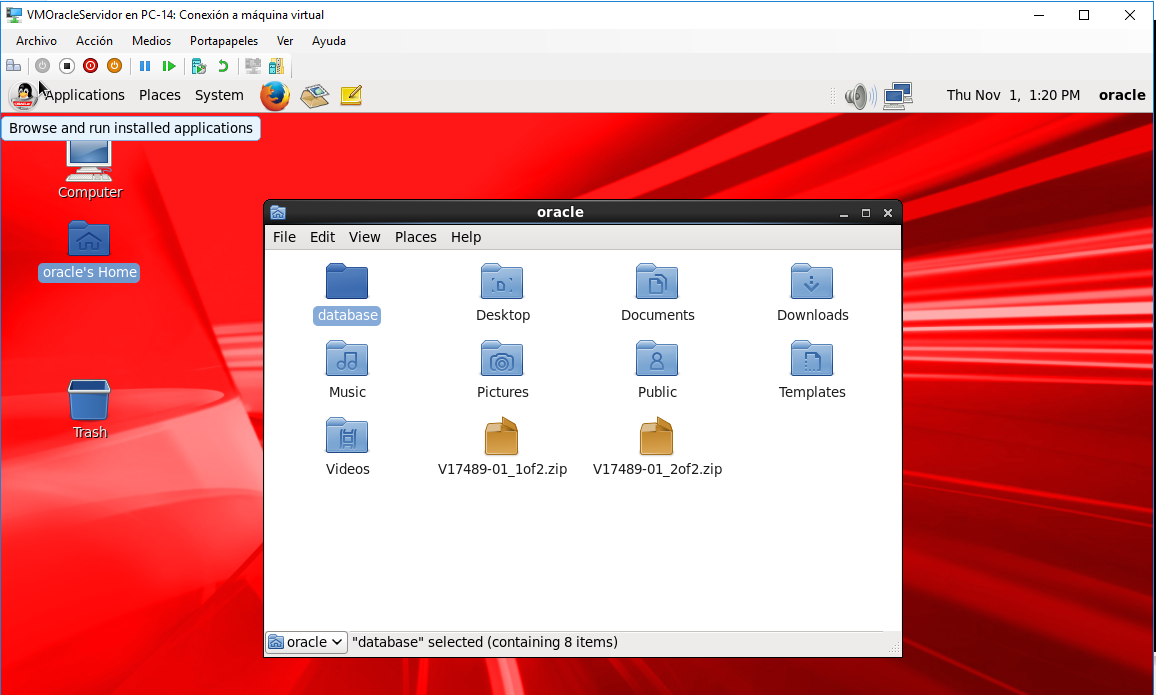
\includegraphics[width=15cm]{./Imagenes/66} 
\end{center} 

\vspace{\baselineskip}

Dentro seleccionamos y abrimos el archivo llamado “runInstaller”.
\begin{center}
	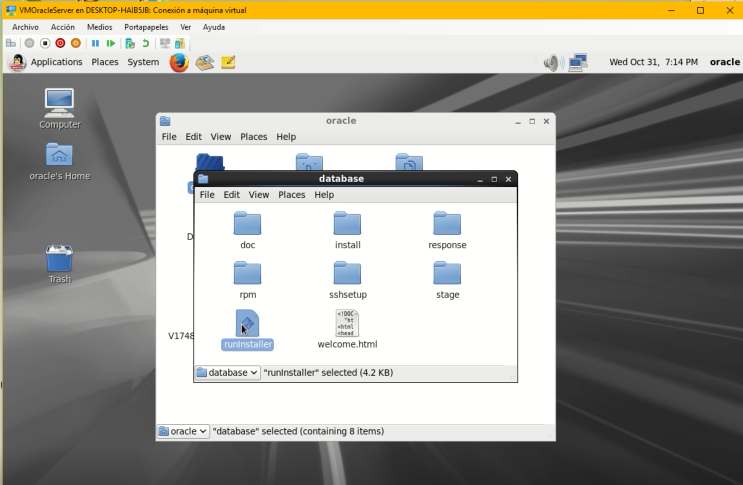
\includegraphics[width=16cm]{./Imagenes/67} 
\end{center} 

\vspace{\baselineskip}

Donde nos aparecerá una ventana de confirmación, en la cual seleccionamos la opción “Run”.
\begin{center}
	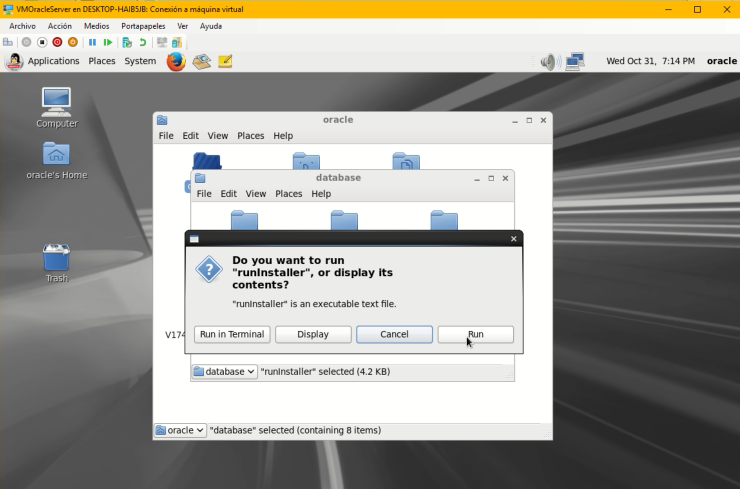
\includegraphics[width=16cm]{./Imagenes/68} 
\end{center} 

\vspace{\baselineskip}

A continuación, se iniciará el programa de instalación de Oracle Database.
\begin{center}
	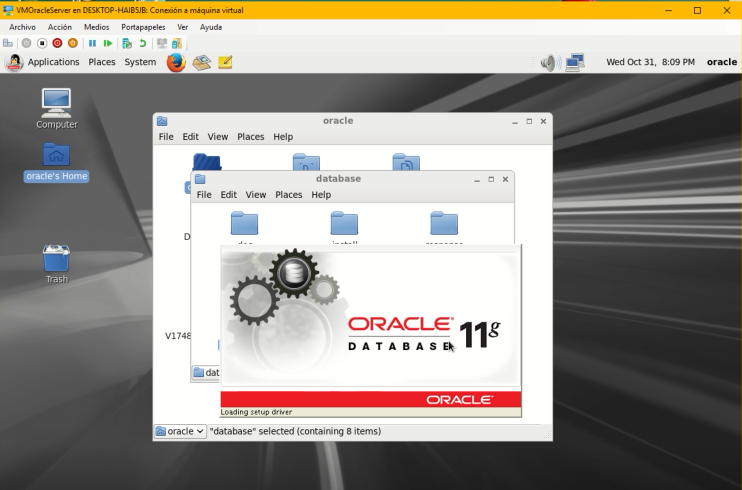
\includegraphics[width=15cm]{./Imagenes/69} 
\end{center} 

\vspace{\baselineskip}

En el cual debemos ingresar un correo electrónico valido, también debemos retirar el check sobre la opción Deseo recibir actualizaciones de seguridad vía Mi Soporte Oracle (I wish to receive security update vía My Oracle Support) y presionar el botón Next (Siguiente).
\begin{center}
	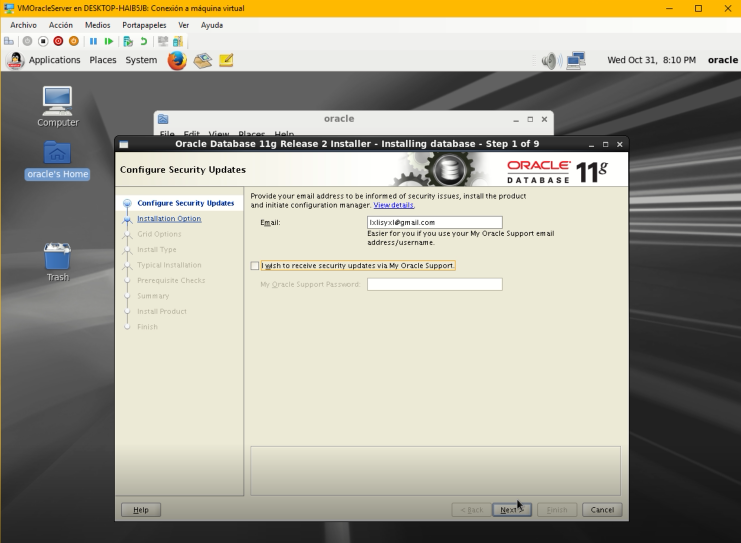
\includegraphics[width=14.8cm]{./Imagenes/70} 
\end{center} 

\vspace{\baselineskip}

Luego, si es que no se tuviese conexión a Internet, se visualizará el siguiente cuadro de dialogo de Fallo en la Conexión (Connection Failed), hacer click en la opción I want to remain uninformed of critical security issues in my configuration (Quiero permanecer desinformado de incidencia de seguridad críticas en mi configuración).
\begin{center}
	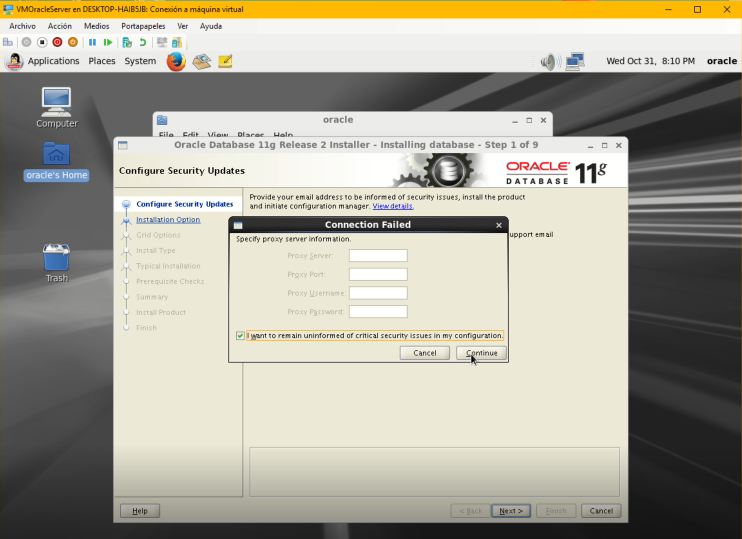
\includegraphics[width=13cm]{./Imagenes/71} 
\end{center}

\vspace{\baselineskip}

Para el siguiente paso se deberá establecer las opciones de instalación, seleccionar la opción Crear y Configurar una base de datos (Create and configure a database) y presionar el botón Next (Siguiente).
\begin{center}
	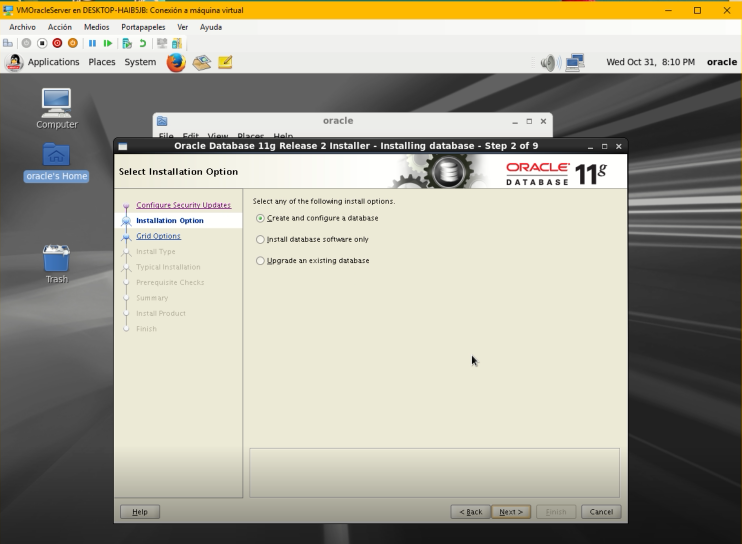
\includegraphics[width=13.3cm]{./Imagenes/72} 
\end{center}

\vspace{\baselineskip}

En el siguiente paso elegimos la Clase de Sistema, para ellos debemos seleccionar la opción Clase Servidor (Server Class), luego presionar el botón Next (Siguiente).
\begin{center}
	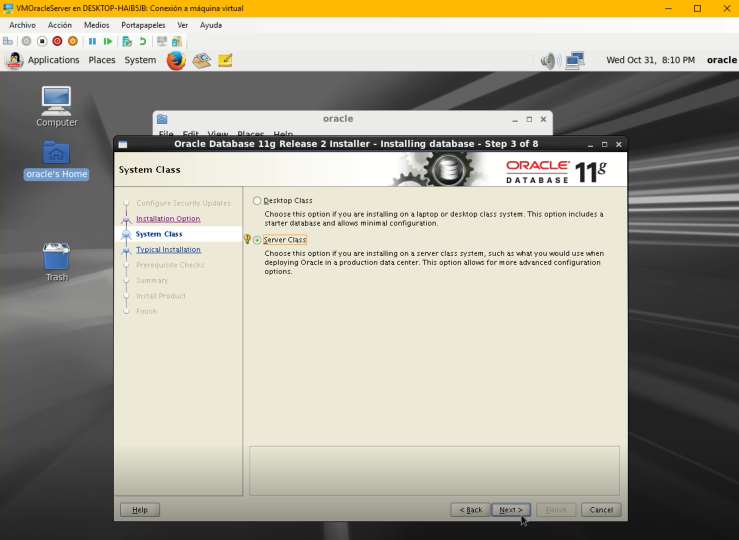
\includegraphics[width=13.3cm]{./Imagenes/73} 
\end{center}

\vspace{\baselineskip}

Para el siguiente paso elegimos las Opciones de Grilla, Selección de Nodo, seleccionar la opción Instalación de base de datos en instancia única (Single instance database installation), seguidamente presionar el botón Next (Siguiente).
\begin{center}
	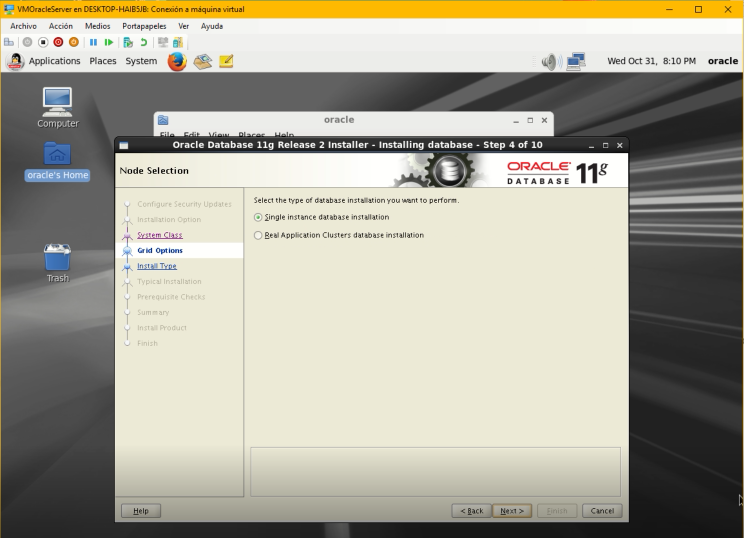
\includegraphics[width=13.3cm]{./Imagenes/74} 
\end{center}

\vspace{\baselineskip}

En el siguiente paso elegimos el Tipo de Instalación, seleccionar Instalación Típica (Typical install) y luego presionar el botón Next (Siguiente).
\begin{center}
	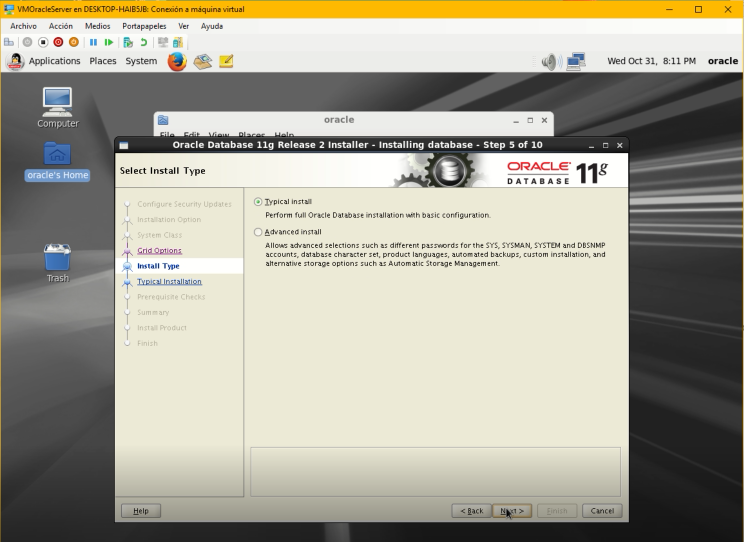
\includegraphics[width=14cm]{./Imagenes/75} 
\end{center}

\vspace{\baselineskip}

Seguidamente en el paso 6 de 10, Configuración de la Instalación Típica, dejar los valores por defecto y establecer la contraseña para los usuarios administrativos (SYS, SYSTEM, SYSMAN y DBSNMP), para cual debe introducir la palabra “oracle” en los cuadros de texto Administrative password (Contraseña de administración) y Confirm Password (Confirmar Contraseña). Una vez terminado esto presionar el botón Next (Siguiente).
	\begin{center}
		\textbf{\large Global DataBase Name: orcl.localdomain \\ Password: oracle
		}		
	\end{center}
\begin{center}
	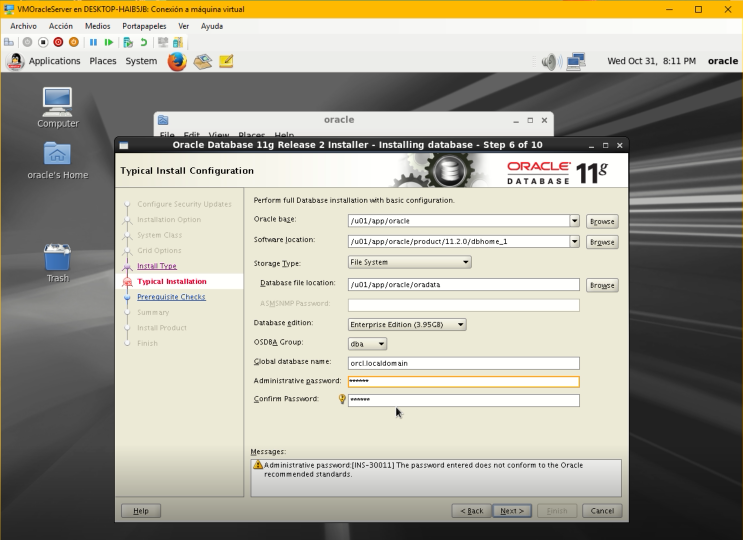
\includegraphics[width=14cm]{./Imagenes/76} 
\end{center}

\vspace{\baselineskip}

Debido a que la contraseña no cumple con los estándares recomendados por Oracle, se visualizará un cuadro de dialogo que solicitará la confirmación si se desea mantener la contraseña introducida, debido a que este es un laboratorio de pruebas la contraseña es suficiente, pero en un ambiente de producción se recomienda utilizar una contraseña más segura. Presionar el botón Yes (Si) en el cuadro de dialogo.
\begin{center}
	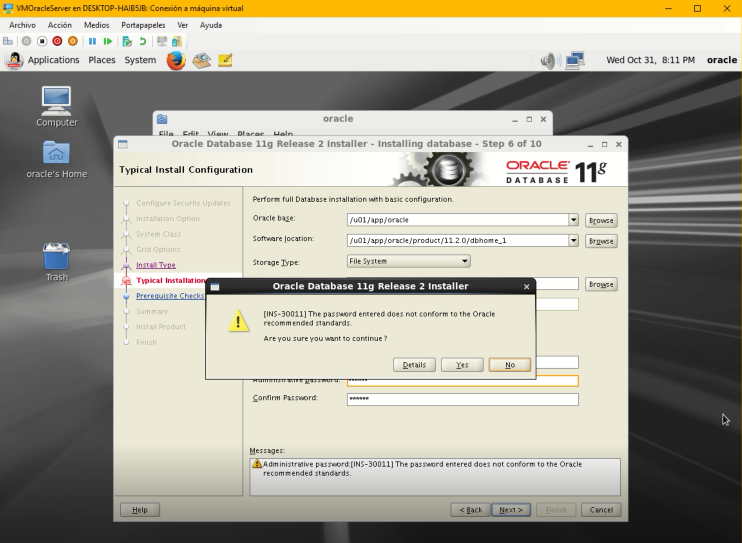
\includegraphics[width=14cm]{./Imagenes/77} 
\end{center}

\vspace{\baselineskip}

En el siguiente paso se deberá establecer la ruta o ubicación donde los productos serán instalados, así como el grupo de usuarios que tiene acceso a realizar modificaciones sobre esta ruta o esta ubicación. Dejar los valores por defecto y presionar el botón Next (Siguiente).
\begin{center}
	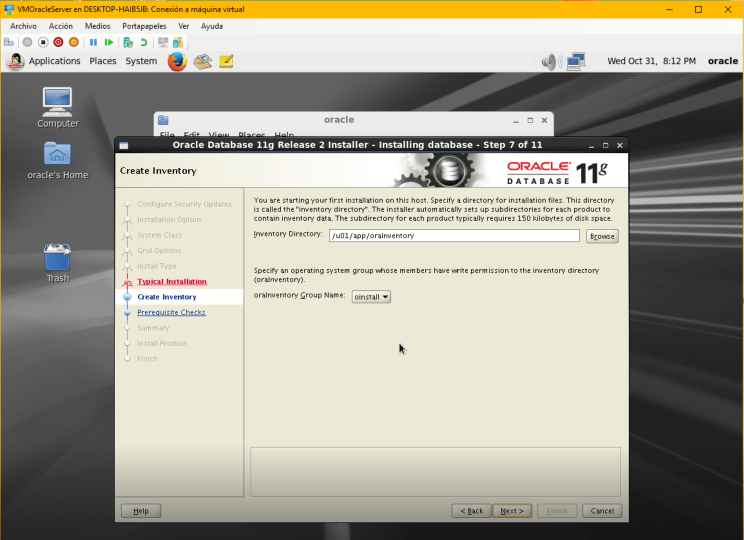
\includegraphics[width=16cm]{./Imagenes/78} 
\end{center}

\vspace{\baselineskip}

A continuación, se el asistente de instalación de Oracle Database realizará la verificación de que todos los pre-requisitos previos a la instalación hayan sido instalados y configurados correctamente. 
Caso contrario si es que hubiese algún inconveniente con los requisitos, con los errores detectados, verificar el detalle y corregir el paso incorrectamente ejecutado.
\begin{center}
	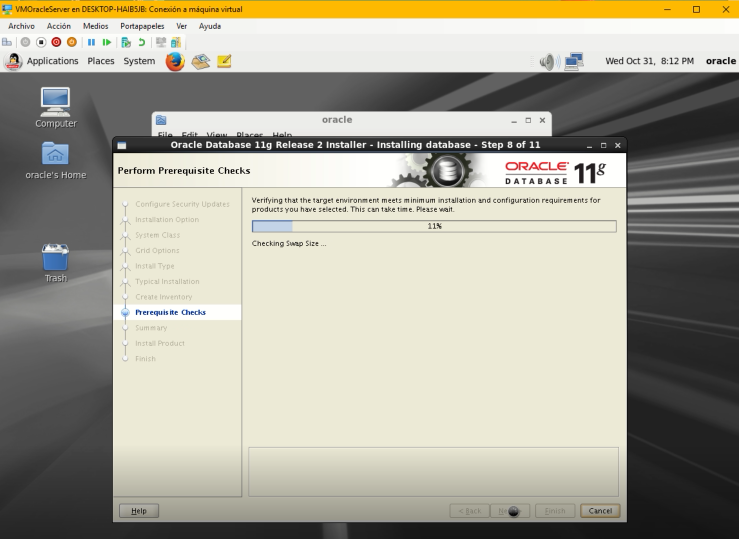
\includegraphics[width=15cm]{./Imagenes/79} 
\end{center}

\vspace{\baselineskip}

Luego nos aparecerá la siguiente ventana en donde seleccionaremos e check de la opción “Ignore All”.
\begin{center}
	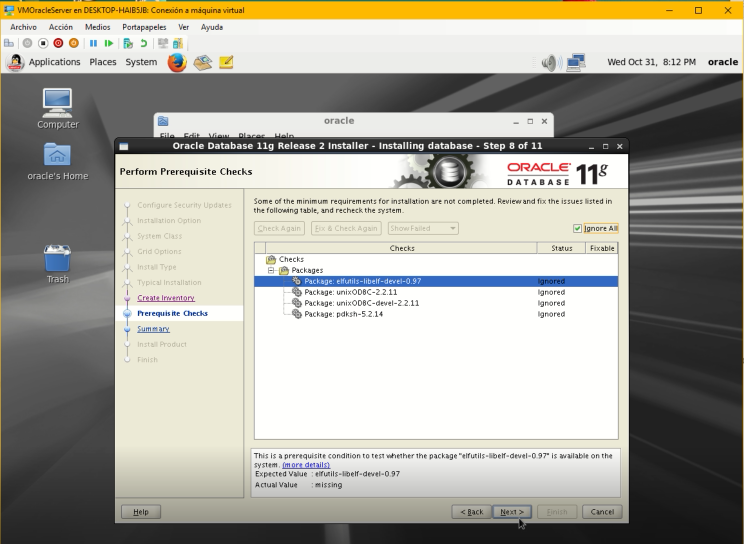
\includegraphics[width=15cm]{./Imagenes/80} 
\end{center}

\vspace{\baselineskip}

Seguidamente aparecerá la pantalla de resumen de configuración previa a la instalación, la cual detalla todos los aspectos seleccionados para la presente instalación, revisar cada línea y luego para iniciar con la instalación presionar el botón Finalizar (Finish).
\begin{center}
	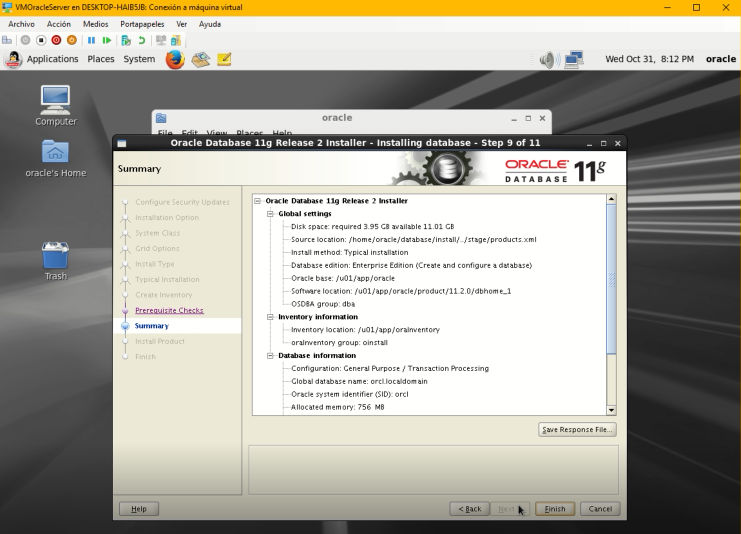
\includegraphics[width=16cm]{./Imagenes/81} 
\end{center}

\vspace{\baselineskip}

En este paso, se visualizará el proceso de instalación, se deberá esperar aproximadamente 15 minutos a que la instalación finalice y complete el 100 por Ciento.
\begin{center}
	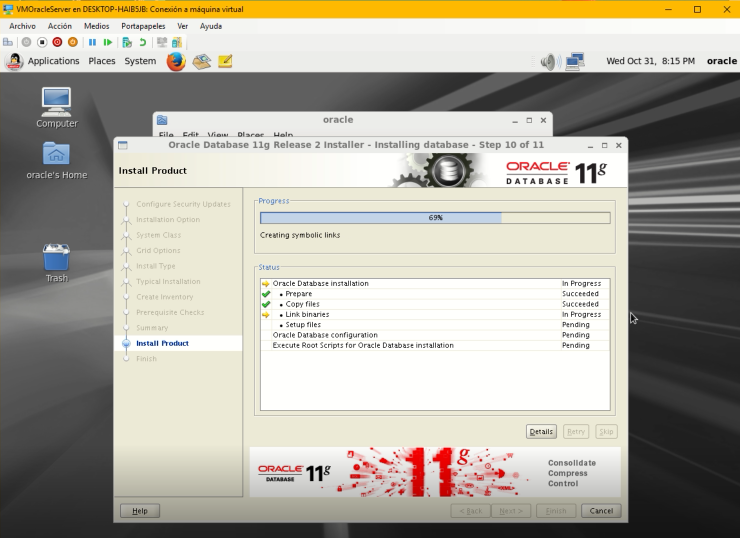
\includegraphics[width=14cm]{./Imagenes/82} 
\end{center}

\vspace{\baselineskip}

Una vez completado el 100 por Ciento de la instalación, se iniciarán de manera automática el asistente de configuración de Base de Datos de Oracle Database. Inmediatamente el Asistente de Configuración de Base de Datos, empezará con la creación de la instancia y luego procederá con la creación de la base de datos del sistema y la base de datos de ejemplo.
\begin{center}
	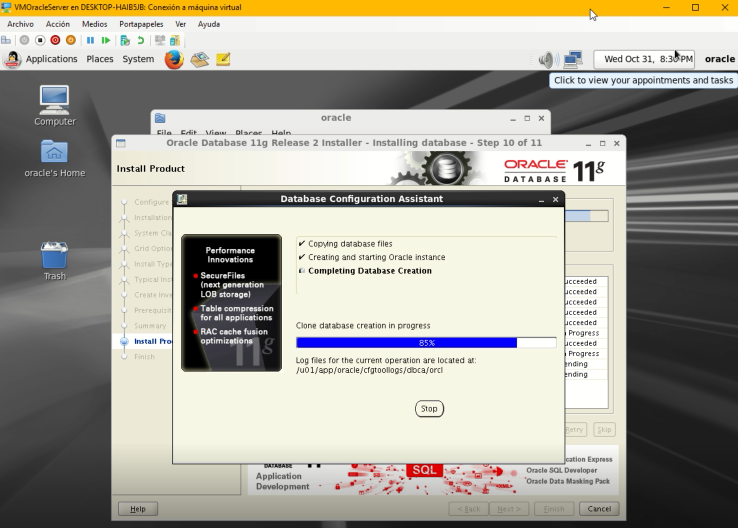
\includegraphics[width=14.5cm]{./Imagenes/83} 
\end{center}

\vspace{\baselineskip}

Una vez finalizada la personalización por parte del Asistente de Configuración de Base de Datos, el instalador de Oracle Database mostrará una pantalla resumen, en donde se indicará la instancia creada y la forma para ingresar a esta, mediante interfaz Web, tomar nota de estos datos y finalmente presionar el botón OK (Aceptar).
\begin{center}
	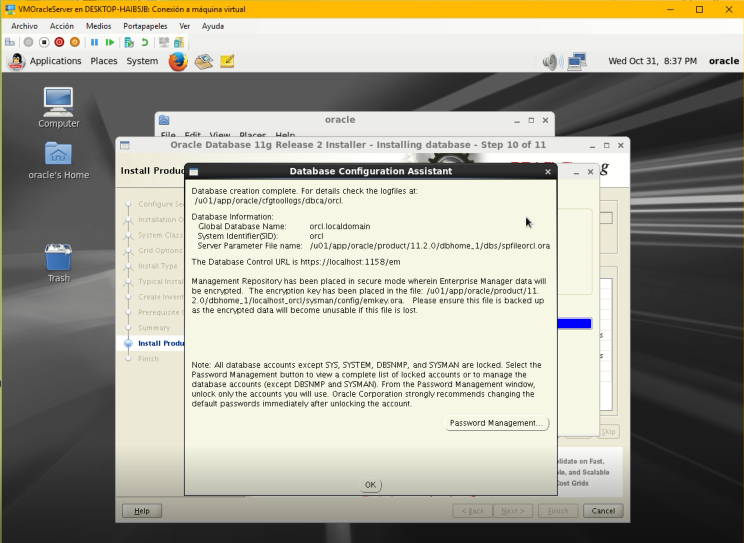
\includegraphics[width=14.5cm]{./Imagenes/84} 
\end{center}

\vspace{\baselineskip}

A continuación, se visualizará una pantalla que solicitará la ejecución de dos scripts que contienen comandos de configuración para el sistema.
\begin{center}
	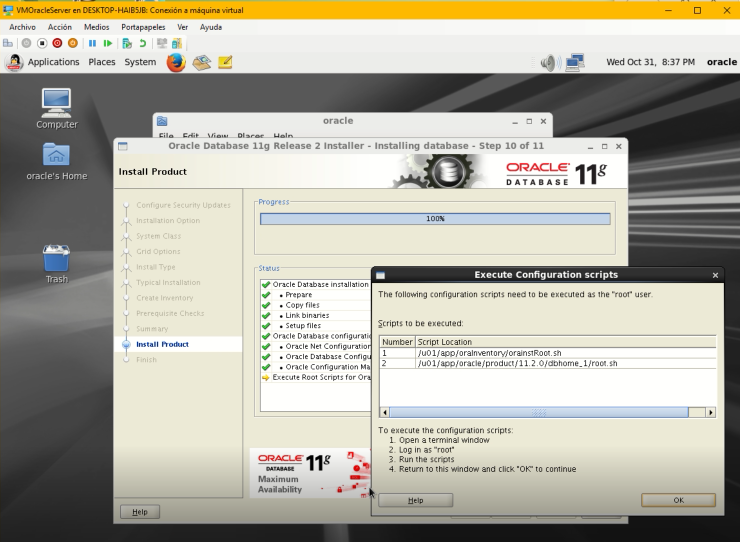
\includegraphics[width=16cm]{./Imagenes/85} 
\end{center}

\vspace{\baselineskip}

Para lo cual será necesario abrir una ventana de Terminal e iniciar sesión como usuario root, ejecutar los comandos y cerrar sesión. Escribir los siguientes comandos en la ventana de Terminal y luego volver a la ventana de ejecución de Comandos del instalador de Oracle Database y presionar el botón OK (Aceptar).

\vspace{\baselineskip}

La siguiente pantalla mostrará la finalización del proceso de instalación. Tomar nota de dirección electrónica (URL) para hacer uso de la herramienta Enterprise Manager Database Control. Finalmente presionar el botón Exit (Salir).

\vspace{\baselineskip}

Como último paso y con la finalidad de verificar de que la instalación ha sido exitosa, iniciar un navegador de Internet (Mozilla u otro similar), e introducir la dirección electrónica de la cual se tomó nota en el paso anterior. Si todo es correcto aparecerá la interfaz de inicio de sesión de la herramienta Enterprise Manager (Administrador Empresarial) de Oracle.